\documentclass[tikz, border=10pt]{standalone}
\usepackage{pgfplots}
\usepgfplotslibrary{groupplots}
\usepackage{amsmath}
\usetikzlibrary{backgrounds, arrows.meta, shapes.geometric}
\pgfplotsset{compat=1.18}

% Define custom colors (more muted for academic slides)
\definecolor{compZero}{HTML}{0D9488}  % Deep Teal
\definecolor{compPole1}{HTML}{2563EB} % Royal Blue
\definecolor{compPole2}{HTML}{475569} % Slate Gray
\definecolor{composite}{HTML}{0F172A} % Navy/Dark Blue
\definecolor{exact}{HTML}{DC2626}     % Muted Red

\begin{document}
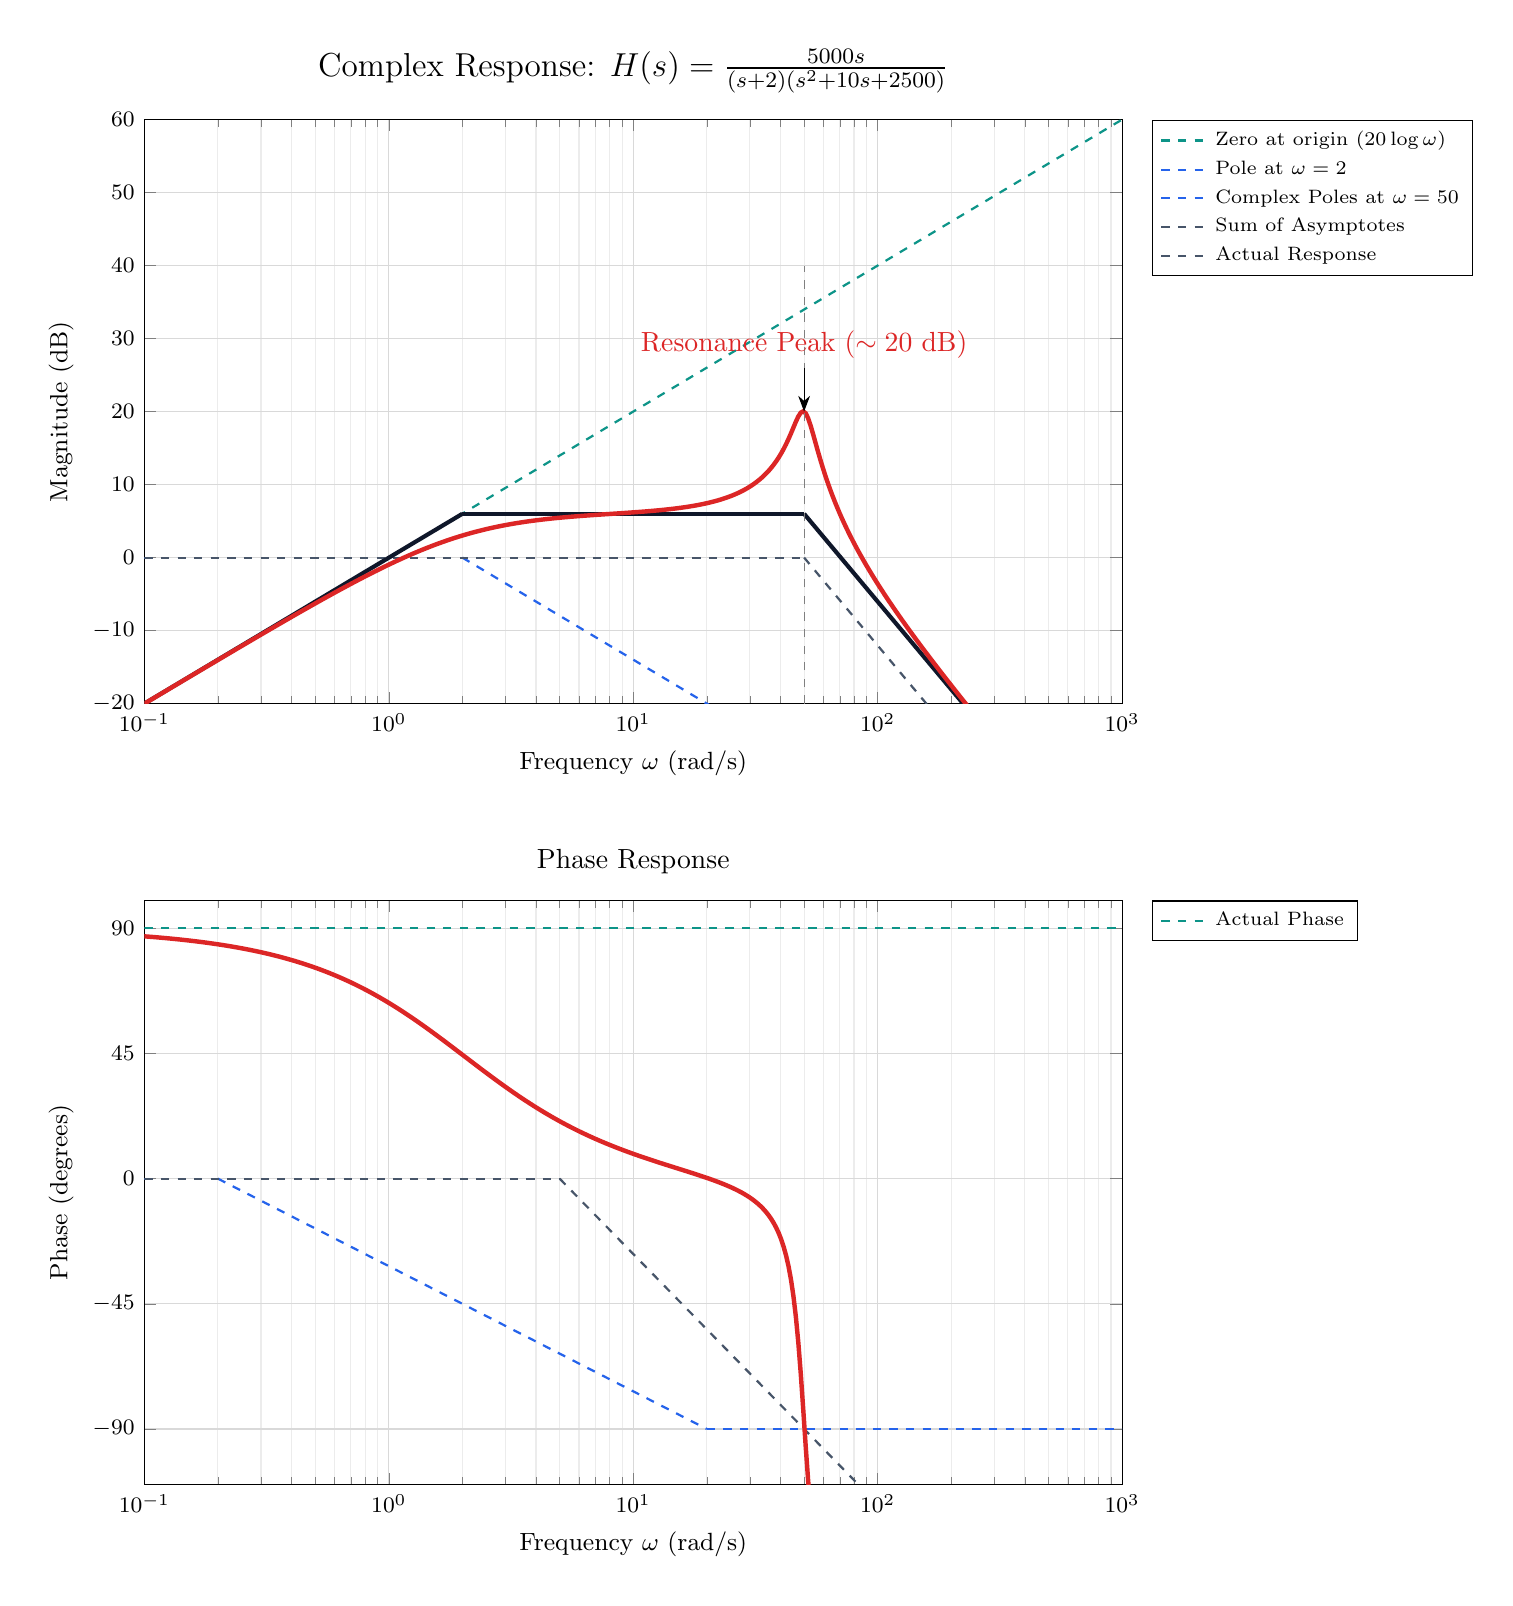
\begin{tikzpicture}[show background rectangle, background rectangle/.style={fill=white}]
    \begin{groupplot}[
        group style={
            group size=1 by 2,
            vertical sep=2.5cm,
        },
        width=14cm, height=9cm,
        xlabel={Frequency $\omega$ (rad/s)},
        xmode=log,
        grid=both,
        xmin=0.1, xmax=1000,
        minor grid style={gray!15},
        major grid style={gray!30},
        tick label style={font=\footnotesize},
        label style={font=\small},
        legend style={font=\scriptsize, cells={anchor=west}}
    ]

    % Magnitude Plot
    \nextgroupplot[
        title={\large Complex Response: $H(s) = \frac{5000s}{(s+2)(s^2 + 10s + 2500)}$},
        ylabel={Magnitude (dB)},
        ymin=-20, ymax=60,
        legend pos=outer north east,
    ]
    
    % Individual Asymptotes
    % 1. Zero at origin: 20 log w
    \addplot[compZero, thick, dashed, domain=0.1:1000] {20*log10(x)};
    \addlegendentry{Zero at origin ($20\log\omega$)}
    
    % 2. Pole at 2: 1/(1+s/2). Corner w=2.
    \addplot[compPole1, thick, dashed, domain=0.1:2] {0};
    \addplot[compPole1, thick, dashed, domain=2:1000] {-20*log10(x/2)};
    \addlegendentry{Pole at $\omega=2$}
    
    % 3. Complex pole pair at 50: 1/(1+s/50+s^2/2500). Corner w=50.
    \addplot[compPole2, thick, dashed, domain=0.1:50] {0};
    \addplot[compPole2, thick, dashed, domain=50:1000] {-40*log10(x/50)};
    \addlegendentry{Complex Poles at $\omega=50$}
    
    % Composite Asymptote
    % w < 2: 20 log w
    % 2 < w < 50: 20 log 2 = 6 dB (constant because zero slope +20 and pole slope -20 cancel)
    % w > 50: 6 - 40 log (w/50)
    \draw[composite, line width=1.5pt] (axis cs: 0.1, -20) -- (axis cs: 2, 6);
    \draw[composite, line width=1.5pt] (axis cs: 2, 6) -- (axis cs: 50, 6);
    \draw[composite, line width=1.5pt] (axis cs: 50, 6) -- (axis cs: 1000, -46);
    \addlegendimage{composite, line width=1.5pt}
    \addlegendentry{Sum of Asymptotes}

    % Exact Curve
    % |H| = 5000w / ( sqrt(4+w^2) * sqrt((2500-w^2)^2 + (10w)^2) )
    \addplot[exact, ultra thick, domain=0.1:1000, samples=400] { 
        20*log10( 5000*x / ( sqrt(4 + x^2) * sqrt( (2500-x^2)^2 + (10*x)^2 ) ) ) 
    };
    \addlegendentry{Actual Response}

    % Annotations
    \draw[dashed, gray] (axis cs: 50, -20) -- (axis cs: 50, 40);
    \node[anchor=south, exact] at (axis cs: 50, 26) {Resonance Peak ($\sim 20$ dB)};
    \draw[{Stealth[length=2mm]}-] (axis cs: 50, 20) -- (axis cs: 50, 26);

    % Phase Plot
    \nextgroupplot[
        title={Phase Response},
        ylabel={Phase (degrees)},
        ymin=-110, ymax=100,
        ytick={90, 45, 0, -45, -90},
        legend pos=outer north east,
    ]

    % Individual Phase Asymptotes
    % 1. Zero at origin: +90
    \addplot[compZero, thick, dashed, domain=0.1:1000] {90};
    
    % 2. Pole at 2: 0 to -90 between 0.2 and 20
    \draw[compPole1, thick, dashed] (axis cs: 0.1, 0) -- (axis cs: 0.2, 0);
    \draw[compPole1, thick, dashed] (axis cs: 0.2, 0) -- (axis cs: 20, -90);
    \draw[compPole1, thick, dashed] (axis cs: 20, -90) -- (axis cs: 1000, -90);
    
    % 3. Complex poles at 50: 0 to -180 between 5 and 500
    \draw[compPole2, thick, dashed] (axis cs: 0.1, 0) -- (axis cs: 5, 0);
    \draw[compPole2, thick, dashed] (axis cs: 5, 0) -- (axis cs: 500, -180);
    \draw[compPole2, thick, dashed] (axis cs: 500, -180) -- (axis cs: 1000, -180);

    % Exact Phase
    % phi = 90 - atan(w/2) - atan2(10w, 2500-w^2)
    \addplot[exact, ultra thick, domain=0.1:1000, samples=400] { 
        90 - atan(x/2) - rad(atan2(10*x, 2500-x^2))*180/pi
    };
    \addlegendentry{Actual Phase}

    \end{groupplot}
\end{tikzpicture}
\end{document}
